\section{Curvature as route dependence of transport}
\label{sec:curvature}

Coherence of distances does not reveal curvature: a sphere and a plane can both carry perfectly coherent metrics.
Curvature appears when one \emph{transports} something, say a frame, along different routes between the same endpoints and compares the results~\cite{Lee1997Riemannian}.
This section makes that idea precise for discrete transports, tests the local-MDS estimator used in our pipeline against it, and shows how curvature can be recovered from the Markov metrics of \cref{sec:sphere}.

\subsection{Holonomy is noncommutation of covariant shifts}
\label{sec:connection}

A tempting slogan is that curvature is ``noncommutativity of local moves''.
Taken literally for planar frames it is false: two rotations of the plane always commute, because $SO(2)$ is abelian.
The correct statement involves operators that move the base point as well as the frame.

Let $X$ carry two commuting translations $u$ and $v$ (for example the two directions of a periodic grid), and suppose each $x\in X$ has a two-dimensional fibre with an orthonormal frame.
Let $A_x$ and $B_x$ be orthogonal matrices transporting the fibres at $ux$ and $vx$ back to $x$.
On the space of sections $s$ (one vector per fibre) define the \emph{covariant shifts}
\begin{equation}
(S_us)(x)=A_x\,s(ux),\qquad (S_vs)(x)=B_x\,s(vx).
\end{equation}
The two routes from $uvx$ back to $x$ have transports $L_x=A_xB_{ux}$ and $M_x=B_xA_{vx}$, and their discrepancy is the square holonomy $H_x=L_xM_x^{-1}$.

\begin{theorem}[Holonomy as a commutator]
\label{thm:commutator}
$\bigl([S_u,S_v]s\bigr)(x)=(H_x-I)\,M_x\,s(uvx)$ for every section $s$.
Hence $S_u$ and $S_v$ commute if and only if $H_x=I$ for every $x$.
If $X$ is finite (so $u,v$ are permutations) and sections carry the $\ell^2$ norm, then $\|[S_u,S_v]\|=\max_x\|H_x-I\|$; if moreover every $H_x$ is a rotation, with angle $\theta_x\in[0,\pi]$, this equals $\max_x 2\sin(\theta_x/2)$ (an orientation-reversing $H_x$ has $\|H_x-I\|=2$ and no rotation angle).
Under independent frame changes $Q_x\in O(2)$, $H_x\mapsto Q_xH_xQ_x^{-1}$ and the commutator is conjugated by an orthogonal map, so $\theta_x$ and the norm are invariant.
\end{theorem}

\provenance{Lean: \lean{covariantShift_commute_iff}, \lean{covariantShift_gauge} and \lean{plaquetteHolonomy_gauge} in \lean{Connection.lean}, for group-valued frame fields acting by their regular action, including abelian groups. Written proof: the linear formula, the norm identity and the angle formula (\cref{app:connection-proof}).}

The commutator is nonzero when the coefficients, evaluated at \emph{different} base points, fail to satisfy $A_xB_{ux}=B_xA_{vx}$, which abelian coefficients do not prevent.
Conversely, constant coefficients that commute with each other, for instance constant rotations, give commuting shifts and trivial holonomy even when each individual transport is a nontrivial rotation, so patchwise framing does not by itself create curvature.
For triangular loops the same idea reads: invertible transports $a\colon x\to y$, $b\colon y\to z$, $c\colon x\to z$ satisfy $ab c^{-1}=1$ if and only if $ab=c$ (\lean{triangleHolonomy_eq_one_iff}), and for orthogonal transports whose triangle holonomy is a rotation by $\theta$, the disagreement between the two-step and the direct route is $\|ab-c\|=2\sin(\theta/2)$.

\paragraph{An exact curved example.}
On the unit sphere with latitude $\phi$ and longitude $\lambda$, the Levi-Civita connection in the frame $(e_\phi,e_\lambda)$ transports along a latitude by the rotation $R(\sin\phi\,\Delta\lambda)$ and along a meridian by the identity.
For the rectangle bounded by latitudes $\phi_0<\phi_1$ and a longitude interval of width $w$, the square holonomy is the rotation by $-w(\sin\phi_1-\sin\phi_0)$, minus the enclosed area.
With $\sin\phi_0=\tfrac14$, $\sin\phi_1=\tfrac12$ and $w=\tfrac14$, the area and the holonomy angle are both exactly $1/16$, and $\|[S_u,S_v]\|=2\sin(1/32)>0$; the flat connection gives zero.
For rectangles of side $h$ around a fixed latitude, the principal angle divided by the area equals $1$ whenever the area is below $\pi$, in particular for all small $h$, while the raw angle tends to zero.
Recovering curvature from shrinking loops therefore requires normalizing by area; a raw angle that vanishes under refinement is not evidence of flatness.

\subsection{The local-MDS and Procrustes estimator}
\label{sec:mds-estimator}

Our pipeline estimates holonomy from a finite metric as follows.
Each macro state and its $k$ nearest neighbours (optionally expanded by one hop) are embedded in the plane by classical multidimensional scaling~\cite{BorgGroenen2005}, keeping the two leading positive eigenvalues.
The transport between two overlapping charts is the orthogonal polar factor of the cross-covariance of their centred overlap coordinates, the orthogonal Procrustes solution~\cite{Schonemann1966}, computed over the full group $O(2)$ because each MDS chart is determined only up to rotation \emph{and} reflection.
Overlaps or cross-covariances of deficient rank are excluded.
For a sampled triangle of neighbouring states the holonomy score is the rotation angle of the product of the three transports; orientation-reversing products have no rotation angle and are counted separately.
By \cref{thm:commutator} and the triangle criterion, these scores are gauge invariant and measure the route disagreement of the estimated discrete connection.
For an exact planar Euclidean metric every full-rank chart is an isometric copy of the plane coordinates, and every triangle holonomy is exactly zero.

\begin{figure}[t]
\centering
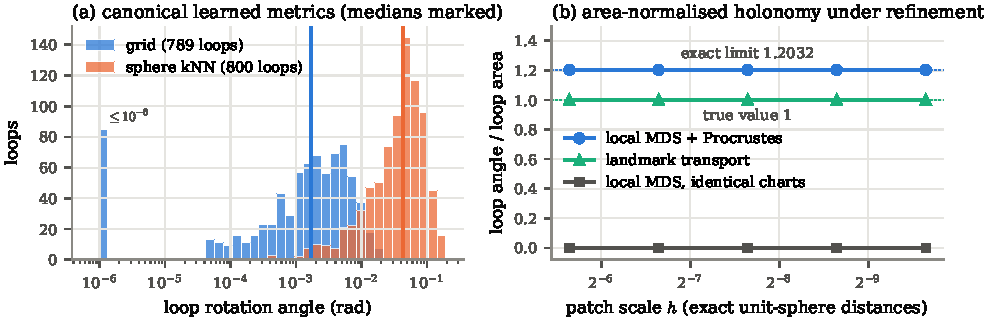
\includegraphics[width=\linewidth]{figures/fig_holonomy.pdf}
\caption{Holonomy estimation. (a) Loop rotation angles on the canonical learned metrics ($m=128$, $\tau=5$; $k=24$ chart neighbours, one-hop expansion, triangles from $8$ nearest neighbours). Medians over all evaluated loops: $0.00169$ (grid) and $0.0428$ (sphere $k$NN). No loop was excluded; the $85$ grid angles below $10^{-6}$ (numerically zero) are collected in the leftmost bin. (b) Exact unit-sphere distances on a fixed $12$-point patch scaled by $h$: the area-normalized output of the local-MDS estimator converges to the exact constant $\approx1.20317$, the same estimator with identical charts returns $0$, and the landmark transport estimator of \cref{sec:transport-repair} returns $1$. Floating computation; the limit constant is exact.}
\label{fig:holonomy}
\end{figure}

\paragraph{Finite separation on the learned metrics.}
On the canonical learned metrics (\cref{fig:holonomy}a), the median triangle angle is $0.00169$ radians on the grid ($789$ triangles) and $0.0428$ on the sphere $k$NN substrate ($800$ triangles), a ratio of about $25$; no triangle was excluded for missing transport or reversed orientation.
The estimator thus separates the two substrates under this fixed protocol.
What it measures is the non-flatness of the estimated connection on two learned metrics that, by \cref{sec:learned}, are not coherent layers.
It is not an estimate of Riemannian curvature, and the next result shows that it could not be one in general.

\begin{theorem}[The local-MDS estimator is not a consistent curvature estimator]
\label{thm:mds-obstruction}
Apply the estimator to exact geodesic distances on the unit sphere, for point configurations obtained by mapping a fixed planar configuration through the exponential map at scale $h\to0$.
\begin{enumerate}[label=(\roman*)]
\item If the three charts of a triangle contain the same point set, their overlaps have full rank, and the second and third eigenvalues of the centred Gram matrix are distinct (which holds for all small $h$), the estimated holonomy is exactly zero. For noncollinear chart centres the enclosed spherical area is positive, so the curvature is missed entirely.
\item For an explicit configuration of $12$ points with $k=8$, the three charts are distinct, every chart and overlap stays uniformly nondegenerate after rescaling coordinates by $1/h$ (cross-covariances by $1/h^2$), and the estimated angle divided by the true spherical area converges to
\begin{equation}
\frac{7884106465972959320549378723}{6552773242191625884795360000}\approx1.20317>\tfrac65 .
\end{equation}
\item Both configurations can be embedded in samples that become dense on the whole sphere without changing the three charts.
\end{enumerate}
\end{theorem}

\provenance{Written proof (\cref{app:mds-proof}): second-order expansion of spherical distances, perturbation of the retained spectral subspace across the gap to the zero eigenvalues, and the first-order polar factor; the limiting constant is computed in exact rational arithmetic. Lean: \lean{triangleHolonomy_common_chart} gives the cancellation in (i). Floating computation: \cref{fig:holonomy}b, $h=2^{-k}/50$ for $k=0,\dots,4$.}

Part (i) holds because identical point sets give the same Gram matrix up to a permutation, so with a strict eigenvalue gap the three charts are gauge copies of one another, whatever the curvature.
Part (ii) shows that the failure is not caused by degenerate charts or reflections: with distinct, well-conditioned charts the bias in the area-normalized output is about $20\%$ in the limit.
The estimator does satisfy a stability bound: for nonsingular cross-covariances $M,N$ with polar factors $U,V$,
$\|U-V\|_F\le2\|M-N\|_F/(\sigma_{\min}(M)+\sigma_{\min}(N))$.
But in charts of size $h$ the coordinate errors induced by curvature are of order $h^3$, which permits transport errors of order $h^2$, exactly the order of curvature times area.
The bound cannot make the area-normalized error vanish, and (ii) shows that it does not.

\subsection{Landmark transport and curvature from Markov metrics}
\label{sec:transport-repair}

If the metric is known to be (close to) that of the unit sphere and three mutually orthogonal landmark points $a_1,a_2,a_3$ are marked, curvature can be recovered consistently.
Each point $i$ is reconstructed as $p_i=r_i/|r_i|$ with $r_i=(\cos d(i,a_1),\cos d(i,a_2),\cos d(i,a_3))$, which recovers its position in the landmark basis exactly for exact spherical distances.
The minimal rotation taking $p$ to $q$,
\begin{equation}
R(p,q)=I+K+\frac{K^2}{1+p\cdot q},\qquad K=\text{the cross-product matrix of }p\times q,
\end{equation}
is parallel transport along the shorter great-circle arc, and tangent frames are obtained by projecting a fixed unit reference vector onto each tangent plane and normalizing.
Around a geodesic triangle of area below $\pi$ the resulting principal loop angle equals the enclosed area, by Stokes' theorem applied to the connection form of the frame.

\begin{theorem}[Quantitative landmark transport]
\label{thm:landmark}
Suppose all measured distances, including those to the landmarks, are within $\epsilon\le1/(2\sqrt3)$ of true unit-sphere distances.
Suppose also that, for both the true and the reconstructed points, the tangential projections of the unit reference vector have length at least $\kappa>0$ and every arc satisfies $1+p\cdot q\ge\gamma>0$.
Then for every geodesic triangle whose true area is below $\pi$
\begin{equation}
\bigl|\text{estimated angle}-\text{true area}\bigr|\;\le\;3\pi\sqrt3\,C\,\epsilon,
\qquad C=4+\frac{16}{\kappa}+\frac4\gamma+\frac2{\gamma^2}.
\end{equation}
\end{theorem}

\provenance{Written proof (\cref{app:landmark-proof}). Lean: \lean{triangle_transport_error} bounds the error of a product of three approximate contractions in a normed ring, and \lean{normalized_angle_error} divides angle error by a positive area.}

Consistency under refinement therefore needs more than metric convergence: the metric error must be small compared with the loop area, $\epsilon/\text{area}\to0$.
The reservoir family of \cref{sec:sphere} supplies exactly this.

\begin{theorem}[Curvature from staged Markov metrics]
\label{thm:markov-curvature}
In the spherical reservoir family, use the normalized metrics $d/t_r$ (values above $\pi$ clipped to $\pi$ for reconstruction only), the three positive axis points as landmarks, and triangles formed by the north landmark and two mesh points at gnomonic coordinates near $(h_r,0)$ and $(0,h_r)$, with $h_r=2^{-r/8}$.
Then the true triangle areas are at least $h_r^2/8$, the margins $\kappa=0.8$ and $\gamma=1.8$ hold for all large $r$, and the landmark estimator satisfies
\begin{equation}
\left|\frac{\text{estimated angle}}{\text{true area}}-1\right|\;\le\;24\pi\sqrt3\,C\,\frac{\epsilon_r}{h_r^2}\;\longrightarrow\;0,
\end{equation}
because $\epsilon_r/h_r^2=4\pi\sqrt2\,2^{-3r/4}+(16+\log_26+3r)\,2^{-r/4}$.
The area-normalized curvature read from the actual staged Markov metrics converges to $1$, the curvature of the unit sphere.
\end{theorem}

\provenance{Written proof (\cref{app:sphere-proof}), combining \cref{thm:sphere}(ii) with \cref{thm:landmark}. Floating computation: three finite end-to-end controls (Markov kernel to metric to transport, reservoir volume $8$, $\beta=64,128,256$, triangle area $\approx0.0196$) give area-normalized angles $1.077$, $1.083$ and $1.033$; these illustrate the pipeline but do not by themselves establish convergence.}

The result uses recognition input that the learned ladders do not provide: the knowledge that the metric is spherical, three marked orthogonal landmarks, and the declared unit $t_r$.
It does not show that an unknown manifold can be recognized from its Markov metric, and it does not reinterpret the finite learned-metric scores above as curvature estimates.
What it does show is that the chain \emph{dynamics $\to$ lens $\to$ likelihood path metric $\to$ transport $\to$ curvature} can be closed with proofs at every link.
